\qs{}{
    How many students have the same mother but different fathers?
}

This counts the number of students who have same mothers but different fathers by joining and comparing two student tables, and the \texttt{DISTINCT} keyword also ensures that each student is counted only once.
\vspace{\baselineskip}

\sol{}
\noindent\line(1, 0){0.89\linewidth}
\begin{verbatim}
SELECT COUNT(DISTINCT s1.stud_id) AS "Students with Same Mothers but Different Fathers" 
FROM student s1
JOIN student s2 ON s1.stud_mother = s2.stud_mother AND s1.stud_father != s2.stud_father;
\end{verbatim}
\noindent\line(1, 0){\linewidth}

\begin{figure}[H]
    \centering
    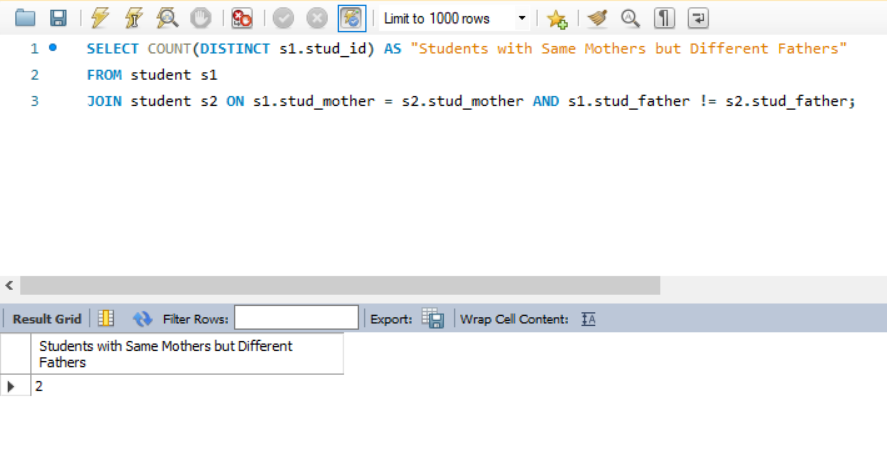
\includegraphics[width=0.7\linewidth]{images/q5.png}
    \caption{Question 5 Query and Output}
\end{figure}
